\documentclass[10pt,a4paper]{article}
\usepackage[T1]{fontenc}
\usepackage{lmodern}
\usepackage{microtype}
\usepackage[margin=2.1cm]{geometry}
\usepackage{amsmath,amssymb}
\usepackage{booktabs,array}
\usepackage{graphicx}
\usepackage{float}
\usepackage{enumitem}
\usepackage{xcolor}
\usepackage[colorlinks=true,linkcolor=blue!50!black,urlcolor=blue!50!black]{hyperref}
\setlist{itemsep=2pt,topsep=3pt}
\emergencystretch=2em

\newcommand{\code}[1]{\texttt{#1}}
\newcommand{\Ds}{D_s}
\newcommand{\Dss}{D_s^*}
\newcommand{\mm}{m^2_\text{miss}}
\newcommand{\Es}{E^*_\mu}
\newcommand{\PV}{P(V_{B_s})}
\newcommand{\sR}{\sigma R}

\newcommand{\finding}[1]{\par\smallskip\noindent\colorbox{blue!6}{\parbox{\dimexpr\linewidth-2\fboxsep}{#1}}\par\smallskip}

\title{$R(D_s)$ signal MC: kinematic-fit schemes, $B_s$ hypotheses\\ and what the BDT gains from each input}
\author{Summary of \code{compare\_fits} \code{cmp\_v1}--\code{cmp\_v3} and the full-statistics \code{hypinfo} study}
\date{3 November 2026}

\begin{document}
\maketitle

\section*{The answers in one page}

Every statement about an input is only meaningful together with \emph{what else is already in the fit}. The table
gives each conclusion with that condition. The sections after it give the evidence.

\begin{center}
\small
\begin{tabular}{>{\raggedright\arraybackslash}p{0.27\textwidth}>{\raggedright\arraybackslash}p{0.33\textwidth}>{\raggedright\arraybackslash}p{0.32\textwidth}}
\toprule
question & answer & condition, evidence \\
\midrule
Which vertex-fit scheme? & \textbf{\code{free}} (no mass constraint). Decided. &
  All four schemes give the same physics within 1\%; the $\phi$ constraint loses 32--35\% of the signal, the
  $\Ds$ constraint 5\% (Sec.~\ref{sec:schemes}). \\
\addlinespace
Which $B_s$ momentum hypothesis? & \textbf{\code{xyz\_bs}} as the primary one. &
  Best alone in every test; \code{coll} is a single variable in disguise (Sec.~\ref{sec:hyp}). \\
\addlinespace
Does \code{coll} add anything? & \textbf{No}, in any configuration. &
  $\le1\%$ on top of \code{xyz\_bs}, with or without other inputs (Sec.~\ref{sec:bdt}). \\
\addlinespace
Does \code{math} add anything? & \textbf{Depends on the other inputs.} &
  BDT with kinematics only: $-7.5\pm0.8\%$ on $\sR(\Ds)$. BDT with context: $-0.7\pm0.3\%$, i.e.\ nothing. Binned
  2D fit: $-11\%$, not yet robust (Sec.~\ref{sec:bdt}, \ref{sec:binned}). \\
\addlinespace
Is that gain specific to \code{math}? & \textbf{No.} &
  The raw track kinematics next to \code{xyz\_bs} give the same gain ($-6.5\%$). \\
\addlinespace
Do the photon hypotheses ($q^2$, $\mm$ with $\Ds\gamma$) add anything? & \textbf{No}, once the photon
  \emph{quality} variables are in. & $-0.4\pm0.3\%$ on top of context. The photon quality variables themselves are
  the largest single gain for $R$ ($-35\%$ in \code{cmp\_v2}). \\
\addlinespace
What does matter? & The \textbf{context} variables (topology, photon quality, kinematics, isolation). &
  $-45\%$ on $\sR(\Ds)$, $-38\%$ on $\sR(\Dss)$, $-15\%$ on $\sigma_{\tau/\mu}$ vs \code{xyz\_bs} alone. \\
\addlinespace
Can the method see a real gain? & \textbf{Yes.} & Two positive controls give $-27\%$ on $\sR(\Ds)$. \\
\bottomrule
\end{tabular}
\end{center}

%=====================================================================
\section{How the comparisons are made}
\label{sec:method}

\paragraph{Samples.} UL18 $B_s\to\Ds^{(*)}\ell\nu$ signal MC (first 500 files), selection: truth-matched signal of the
four channels, correct particle species, trigger path and muon match, one candidate per event.

\begin{center}
\small
\begin{tabular}{llrrrr}
\toprule
study & input & $\Ds\mu\nu$ & $\Dss\mu\nu$ & $\Ds\tau\nu$ & $\Dss\tau\nu$ \\
\midrule
\code{cmp\_v1}, \code{cmp\_v2} & \code{rds\_prod.root}, 17\% read & 114\,684 & 347\,552 & 5\,986 & 15\,680 \\
\code{cmp\_v3} & dsc production, 27\% of 239 chunks & 114\,531 & 346\,149 & 5\,780 & 15\,543 \\
\code{hypinfo\_full} & dsc production, all 500 chunks & 929\,478 & 2\,822\,510 & 48\,024 & 126\,751 \\
\bottomrule
\end{tabular}
\end{center}

\paragraph{Figure of merit.} Every number is the expected relative uncertainty from a \emph{binned Poisson fit of the
four signal yields with perfect templates}: no background, no systematics, no template statistics. The $\tau$ channels
are weighted to $R(\Ds)=0.299$, $R(\Dss)=0.244$ and the sample is scaled to $10^5$ $\Ds\mu\nu$. Three quantities:
\begin{itemize}
\item $\sigma_{\tau/\mu}$: two yields ($\Ds$ and $\Dss$ merged), so it measures $\tau/\mu$ separation alone;
\item $\sR(\Ds)$, $\sR(\Dss)$: four yields, so they also need $\Ds$ told apart from $\Dss$. This is the hard part:
  $\sR(\Ds)$ is 15--28 times its counting limit, $\sigma_{\tau/\mu}$ only about 6 times.
\end{itemize}
These numbers \emph{rank} inputs; they are not the sensitivity of the analysis.

\paragraph{What is binned.} For observables (Sec.~\ref{sec:hyp}, \ref{sec:binned}): equal-population bins, 12 per axis
in 2D, 6 in 3D. For a BDT (Sec.~\ref{sec:bdt}): the four-class output is reduced to the plane
$p_\tau = P(\Ds\tau)+P(\Dss\tau)$, $p_{*} = P(\Dss\mu)+P(\Dss\tau)$, binned in $10\times10$ (``b10'', \code{cmp\_v2}) or
$20\times20$ (``b20'', \code{hypinfo}) equal-population bins. b10 loses about 10\% against b20. An unbinned version was
tried and found unstable; it is not used.

\finding{\textbf{How precise the figures are.} Between two runs on different events, $\sR(\Ds)$ moves by 5--12\%
(\code{cmp\_v2} vs \code{cmp\_v3}). Between two input sets on the \emph{same} events, a paired bootstrap gives
uncertainties of 0.1--1\%. So: differences within one study are meaningful at the per-cent level; absolute values and
differences between studies are not, below $\approx10\%$.}

%=====================================================================
\section{Fit schemes}
\label{sec:schemes}

Four kinematic-fit schemes are run for every candidate. They differ only in the mass constraints:

\begin{center}
\small
\begin{tabular}{lccl}
\toprule
scheme & $m(KK)=m_\phi$ & $m(KK\pi)=m_{\Ds}$ & note \\
\midrule
\code{cons} & yes & yes & \\
\code{phic} & yes & no & the AN choice \\
\code{dsc}  & no  & yes & added for \code{cmp\_v3} \\
\code{free} & no  & no  & \textbf{chosen} \\
\bottomrule
\end{tabular}
\end{center}

\begin{table}[H]
\centering\small
\caption{Fit quality on truth-matched signal ($\mu$ channels), \code{cmp\_v3}. Vertex cuts: $P(V_\phi)>1\%$ and
$P(V_{\Ds})>1\%$. A calibrated fit has $\chi^2/\text{ndf}\approx1$ and 1\% of candidates below $P=1\%$.}
\begin{tabular}{lcccccc}
\toprule
scheme & $V_\phi$ $\chi^2/\text{ndf}$ & $V_\phi$ $P<1\%$ & $V_{\Ds}$ $\chi^2/\text{ndf}$ & $V_{\Ds}$ $P<1\%$ &
  vertex-cut efficiency & $p_T(\Ds)$ $\sigma_{68}$ \\
\midrule
\code{cons} & 9.98 & 0.319 & 3.33 & 0.100 & 0.645 & 0.56\% \\
\code{phic} & 9.98 & 0.319 & 1.06 & 0.006 & 0.679 & 1.02\% \\
\code{dsc}  & 0.94 & 0.005 & 2.45 & 0.046 & 0.950 & 0.46\% \\
\code{free} & 0.94 & 0.005 & 0.93 & 0.001 & \textbf{0.995} & 0.80\% \\
\bottomrule
\end{tabular}
\end{table}

\begin{itemize}
\item \textbf{The $\phi$ constraint is wrong by construction.} The $K^+K^-$ mass spread is dominated by the $\phi$
  natural width ($\Gamma_\phi\approx4.2$\,MeV), which a constraint built on track errors ignores. Its $\chi^2$ term
  averages $\approx19$ per degree of freedom. With the $P(V_\phi)$ cut it removes a third of the signal. It also pulls
  the kaons: $m(\Ds)$ resolution 13.1 vs 10.6\,MeV and $p_T(\Ds)$ 1.02\% vs 0.80\% in \code{phic} vs \code{free}.
\item \textbf{The $\Ds$ constraint is mildly miscalibrated:} its term averages $\approx4$ instead of 1, and
  $P(V_{\Ds})>1\%$ removes 5\% of the signal. The mass-uncertainty demonstrator (separate note, 778k truth-matched
  candidates) explains it: $(m_{KK\pi}-m_{\Ds})/\sigma_m$ from the track covariances has $\langle\text{pull}^2\rangle=4.3$,
  of which the Gaussian core contributes only $1.15^2$; the rest is non-Gaussian tails (3.4\% beyond $3\sigma$, 1\%
  beyond $5\sigma$), partly FSR. Rescaling the momentum errors would not fix it. (The ``57\% fail'' quoted from the smoke test in \code{cmp\_v2} was over all
  candidates, combinatorial ones included; it does not describe signal.)
\item \textbf{Both losses are equal in the four channels}, so they do not bias $R$; they only cost statistics
  ($\sqrt{0.995/0.65}\approx1.24$ in precision for the $\phi$ constraint).
\item \textbf{The physics is the same in every scheme.} The $B_s$ momentum is uncertain at 10--20\% (direction from the
  vertices, magnitude from the visible momentum); a better $\Ds$ momentum ($<1\%$ in every scheme) does not show:
\end{itemize}

\begin{table}[H]
\centering\small
\caption{\code{xyz\_bs} observables per scheme, \code{cmp\_v3}. 3D: binned $(q^2,\mm,\Es)$. BDT: \code{xyz\_bs}
observables + topology + photon + common, 4 folds, b10.}
\begin{tabular}{lcc|ccc|ccc}
\toprule
 & \multicolumn{2}{c|}{$\sigma_{68}$ resolution} & \multicolumn{3}{c|}{3D binned fit} & \multicolumn{3}{c}{BDT} \\
scheme & $q^2$ [GeV$^2$] & $\mm$ [GeV$^2$] & $\sigma_{\tau/\mu}$ & $\sR(\Ds)$ & $\sR(\Dss)$ & $\sigma_{\tau/\mu}$ & $\sR(\Ds)$ & $\sR(\Dss)$ \\
\midrule
\code{cons} & 1.753 & 0.917 & 0.0861 & 0.699 & 0.265 & 0.0775 & 0.436 & 0.197 \\
\code{phic} & 1.765 & 0.921 & 0.0863 & 0.698 & 0.264 & 0.0777 & 0.438 & 0.196 \\
\code{dsc}  & 1.744 & 0.910 & 0.0860 & 0.693 & 0.263 & 0.0772 & 0.436 & 0.196 \\
\code{free} & 1.758 & 0.913 & 0.0862 & 0.697 & 0.264 & 0.0773 & 0.431 & 0.194 \\
\bottomrule
\end{tabular}
\end{table}

\finding{\textbf{Scheme:} \code{free}. Same physics as every other scheme within 1\%, and 99.5\% of the signal
through the vertex cuts against 95\% (\code{dsc}) and 65--68\% (\code{cons}, \code{phic}). A BDT fed with the inputs of
all four schemes together (215 features) gains nothing either.}

%=====================================================================
\section{$B_s$ momentum hypotheses}
\label{sec:hyp}

The $B_s$ momentum is not measured; four hypotheses build it from the visible $\Ds\mu$ and the PV$\to V_{B_s}$
direction, and every observable ($q^2$, $\mm$, $\Es$, angles, \dots) is computed in each.

\begin{center}
\small
\begin{tabular}{l>{\raggedright\arraybackslash}p{0.62\textwidth}}
\toprule
\code{xyz\_bs} & direction PV$\to V_{B_s}$, magnitude $|p_{B_s}|=|p_{\Ds\mu}|\,m_{B_s}/m_{\Ds\mu}$ \\
\code{coll} & along the visible $\Ds\mu$ momentum, same magnitude \\
\code{math1}, \code{math2} & the two analytic solutions for one massless neutrino and the PV$\to V_{B_s}$ direction;
  $\mm=0$ by construction; real for 68--88\% of candidates \\
\code{math\_oracle} & the \code{math} solution closer to the truth (a positive control, not usable in data) \\
\bottomrule
\end{tabular}
\end{center}

\begin{table}[H]
\centering\small
\caption{Per hypothesis, \code{free} scheme, 3D binned fit $(q^2,\mm,\Es)$, \code{cmp\_v1}.}
\begin{tabular}{lcccccc}
\toprule
hypothesis & $q^2$ $\sigma_{68}$ [GeV$^2$] & $q^2$ bias & $\Es$ $\sigma_{68}$ & $\sigma_{\tau/\mu}$ & $\sR(\Ds)$ & $\sR(\Dss)$ \\
\midrule
\code{xyz\_bs}  & 1.75 & $-0.02$ & 0.164 & \textbf{0.085} & \textbf{0.73} & \textbf{0.30} \\
\code{math1}    & 2.20 & $+0.84$ & 0.173 & 0.102 & 0.81 & 0.35 \\
\code{math\_avg} & 2.11 & $+0.42$ & 0.169 & 0.102 & 0.81 & 0.37 \\
\code{math2}    & 2.56 & $-0.07$ & 0.201 & 0.111 & 1.24 & 0.57 \\
\code{coll}     & 2.22 & $+1.12$ & 0.228 & 0.112 & 7.6 & 2.9 \\
\midrule
\code{math\_oracle} & 1.51 & $+0.28$ & 0.111 & 0.104 & 0.65 & 0.29 \\
generator level & -- & -- & -- & 0.045 & 0.24 & 0.10 \\
\bottomrule
\end{tabular}
\end{table}

\begin{itemize}
\item \textbf{\code{coll} is one variable.} With $p_{B_s}\propto p_{\Ds\mu}$, every invariant depends on $m(\Ds\mu)$
  only: its $q^2$, $\mm$, $\Es$ are 100\% rank-correlated, and a 2D/3D fit cannot separate $\Ds$ from $\Dss$.
\item \textbf{\code{math} loses $\mm$}, the strongest single $\tau/\mu$ variable ($\mm$ of \code{xyz\_bs} alone gives
  $\sigma_{\tau/\mu}=0.081$). It reconstructs other quantities better than \code{xyz\_bs}: $p_T(B_s)$, $p_T^\text{miss}$,
  the angles. That is why it was worth testing as an \emph{additional} input (Sec.~\ref{sec:bdt}).
\item The reconstruction loses a factor $\approx1.9$ in $\sigma_{\tau/\mu}$ and $\approx3$ in $\sR(\Ds)$ relative to
  generator level.
\end{itemize}

%=====================================================================
\section{BDT performance versus inputs}
\label{sec:bdt}

\paragraph{Set-up.} One four-class gradient-boosted classifier (scikit-learn \code{HistGradientBoosting}, balanced
classes, out-of-fold predictions from 4 folds) per input set, \code{free} scheme. Two campaigns:

\begin{center}
\small
\begin{tabular}{lll}
\toprule
 & \code{cmp\_v2} (ablation) & \code{hypinfo\_full} \\
\midrule
events & 120k per $\mu$ channel, all $\tau$ ($\approx6$k $\Ds\tau$) & everything (48k $\Ds\tau$) \\
training & stopped after $\approx45$ iterations & to convergence (200--2000 iterations) \\
binning of the output plane & $10\times10$ & $20\times20$ \\
uncertainty & none (scatter $\approx1$\%) & paired bootstrap, 50 replicas \\
\bottomrule
\end{tabular}
\end{center}

\paragraph{The input groups.} Each hypothesis contributes the same 9 observables computed in its $B_s$ rest frame:
$q^2$, $\mm$, $p_T^\text{miss}$, $\Es$, $E^\#_\mu$, $\cos\theta(\phi,\Ds)$, $\cos\theta(\mu,W)$, $\chi$, $p_T(B_s)$.

\begin{center}
\small
\begin{tabular}{lr>{\raggedright\arraybackslash}p{0.7\textwidth}}
\toprule
group & $n$ & content \\
\midrule
\code{xyz} & 9 & the 9 observables of \code{xyz\_bs} (\code{q3}: only $q^2$, $\mm$, $\Es$) \\
\code{coll} & 9 & the same for \code{coll} \\
\code{math} & 18 & the same for \code{math1} and \code{math2} \\
\code{raw} & 13 & $p_T$, $\eta$, $\Delta\phi$ to the flight direction of $K_1$, $K_2$, $\pi$, $\mu$; $\eta$ of the flight
  direction \\
\code{inv} & 9 & $|p_{\Ds}|$, $|p_\mu|$, $m(KK\pi)$, $m(KK)$, $\cos(\Ds,\mu)$, $\cos(\Ds,\text{flight})$,
  $\cos(\mu,\text{flight})$, $(\vec p_{\Ds}\times\vec p_\mu)\cdot\hat d$, $\cos\theta(K,\pi)$ \\
\code{ctx} (context) & 29 & \emph{topology} (11): $\mu$--$\Ds$ DOCA and significance, $\mu$ POCA along $\Ds$, $\mu$ 3D IP
  significance, $\mu$ distance to the $B_s$ direction, $\PV$, $B_s$ and $\Ds$ flight significances, $m_\text{corr}$,
  $p_\perp$, $\cos\theta(K,\pi)$; \emph{photon quality} (3): $p_T(\gamma)$, $\Delta m$, $E_\text{coll}/p_T$;
  \emph{common} (15): masses, $\Delta R$'s, track $p_T$'s, $\mu$ $\eta$, $\mu$ IP significances, isolations \\
\code{$\gamma$hyp} & 4 & $q^2$ and $\mm$ with $\Ds\gamma$ in place of $\Ds$, for \code{xyz\_bs} and \code{coll} \\
\bottomrule
\end{tabular}
\end{center}

\paragraph{Positive controls.} To show that the test can detect information when it is there, two sets add an input
that is known to carry some: the truth-picked \code{math} solution (\code{oracle}), and the generator $q^2$ smeared by
1\,GeV$^2$.

\begin{figure}[H]
\centering
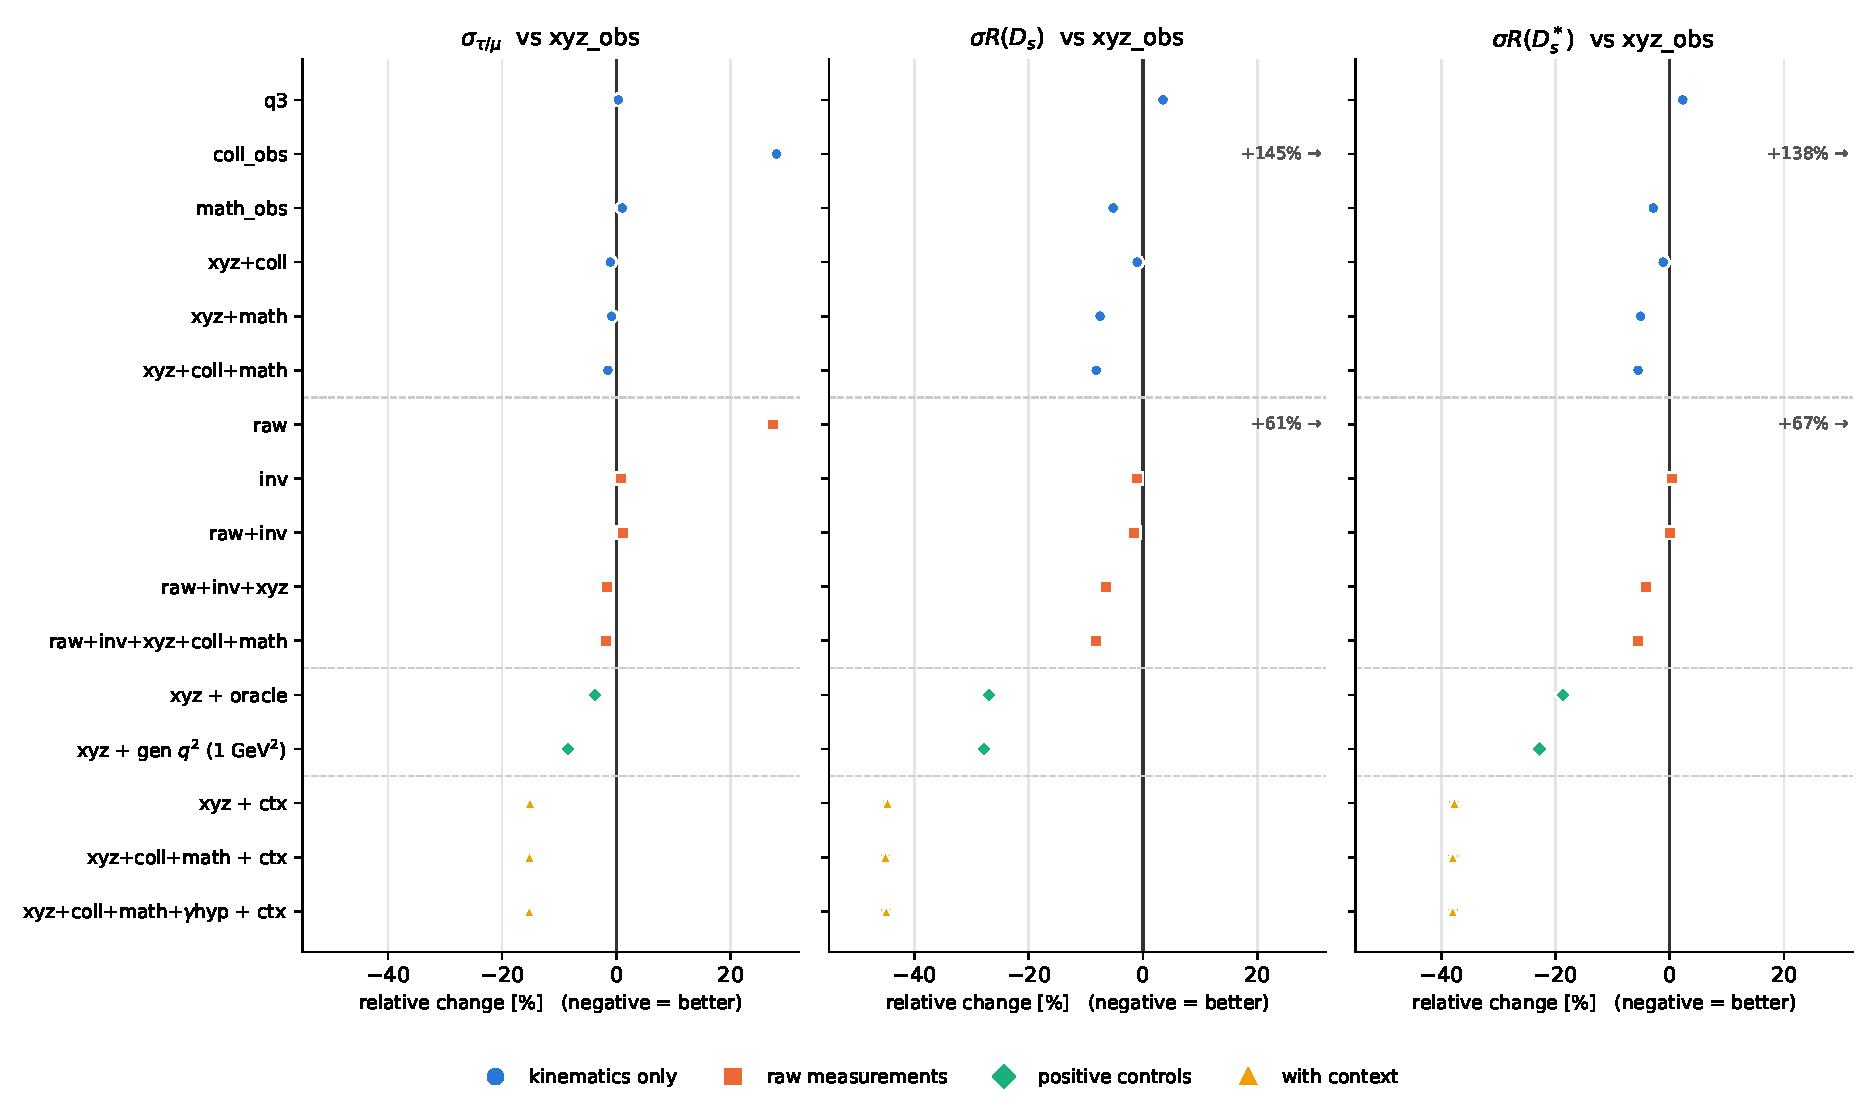
\includegraphics[width=\textwidth]{bdt_gain.pdf}
\caption{Change of the expected precision relative to the BDT on the 9 \code{xyz\_bs} observables, on the same events
(\code{hypinfo\_full}, b20). Error bars: paired bootstrap, mostly smaller than the markers. Off-scale values are printed
at the right edge.}
\label{fig:gain}
\end{figure}

\begin{table}[H]
\centering\scriptsize
\caption{All \code{hypinfo\_full} BDTs: absolute precision (b20), out-of-fold log-loss (lower is better), and the change
relative to \code{xyz\_obs} in per cent.}
\begin{tabular}{lr|ccc|c|ccc}
\toprule
 & & \multicolumn{3}{c|}{expected precision (20$\times$20 bins)} & & \multicolumn{3}{c}{change vs \code{xyz\_obs} (paired bootstrap)} \\
inputs & $n$ & $\sigma_{\tau/\mu}$ & $\sigma R(\Ds)$ & $\sigma R(\Dss)$ & log-loss & $\tau/\mu$ & $R(\Ds)$ & $R(\Dss)$ \\
\midrule
\multicolumn{9}{l}{\emph{reference}} \\
\quad xyz\_obs & 9 & 0.0771 & 0.579 & 0.245 & 1.0944 & -- & -- & -- \\
\multicolumn{9}{l}{\emph{kinematics only}} \\
\quad q3 & 3 & 0.0774 & 0.599 & 0.251 & 1.0969 & $+0.4\pm0.1$ & $+3.5\pm0.8$ & $+2.3\pm0.7$ \\
\quad coll\_obs & 9 & 0.0988 & 1.419 & 0.583 & 1.1912 & $+28.0\pm0.3$ & $+145.1\pm9.9$ & $+137.7\pm8.8$ \\
\quad math\_obs & 18 & 0.0779 & 0.549 & 0.238 & 1.0958 & $+1.1\pm0.1$ & $-5.2\pm1.0$ & $-2.9\pm0.9$ \\
\quad xyz+coll & 18 & 0.0763 & 0.573 & 0.243 & 1.0943 & $-1.0\pm0.0$ & $-1.0\pm0.5$ & $-1.1\pm0.4$ \\
\quad xyz+math & 27 & 0.0765 & 0.535 & 0.233 & 1.0889 & $-0.8\pm0.1$ & $-7.5\pm0.8$ & $-5.1\pm0.7$ \\
\quad xyz+coll+math & 36 & 0.0760 & 0.531 & 0.232 & 1.0872 & $-1.5\pm0.1$ & $-8.2\pm0.8$ & $-5.5\pm0.7$ \\
\multicolumn{9}{l}{\emph{raw measurements}} \\
\quad raw & 13 & 0.0982 & 0.930 & 0.409 & 1.2082 & $+27.4\pm0.3$ & $+60.7\pm3.3$ & $+66.6\pm3.1$ \\
\quad inv & 9 & 0.0777 & 0.572 & 0.246 & 1.1078 & $+0.8\pm0.1$ & $-1.1\pm1.0$ & $+0.4\pm0.9$ \\
\quad raw+inv & 22 & 0.0780 & 0.570 & 0.246 & 1.1102 & $+1.1\pm0.1$ & $-1.5\pm0.9$ & $+0.1\pm0.8$ \\
\quad raw+inv+xyz & 31 & 0.0759 & 0.541 & 0.235 & 1.0874 & $-1.6\pm0.1$ & $-6.5\pm0.8$ & $-4.2\pm0.7$ \\
\quad raw+inv+xyz+coll+math & 58 & 0.0758 & 0.531 & 0.232 & 1.0857 & $-1.8\pm0.1$ & $-8.3\pm0.8$ & $-5.6\pm0.7$ \\
\multicolumn{9}{l}{\emph{positive controls}} \\
\quad xyz + oracle & 18 & 0.0743 & 0.423 & 0.199 & 1.0683 & $-3.7\pm0.1$ & $-27.0\pm0.9$ & $-18.7\pm0.8$ \\
\quad xyz + gen.\ $q^2$ smeared & 10 & 0.0706 & 0.417 & 0.189 & 1.0578 & $-8.5\pm0.1$ & $-27.9\pm0.7$ & $-22.8\pm0.7$ \\
\multicolumn{9}{l}{\emph{with context}} \\
\quad xyz + ctx & 38 & 0.0655 & 0.320 & 0.153 & 1.0308 & $-15.1\pm0.1$ & $-44.7\pm0.8$ & $-37.7\pm0.8$ \\
\quad xyz+coll+math + ctx & 65 & 0.0654 & 0.318 & 0.152 & 1.0338 & $-15.2\pm0.1$ & $-45.1\pm0.8$ & $-38.0\pm0.8$ \\
\quad xyz+coll+math+$\gamma$-hyp + ctx & 69 & 0.0653 & 0.319 & 0.152 & 1.0306 & $-15.3\pm0.1$ & $-45.0\pm0.8$ & $-38.0\pm0.8$ \\
\bottomrule
\end{tabular}

\end{table}

\subsection*{Reading the results in four steps}

\begin{enumerate}[label=\textbf{\arabic*.}]
\item \textbf{Kinematics only, no context} (blue in Fig.~\ref{fig:gain}). \code{coll} adds 1\%. \code{math} adds
  $7.5\pm0.8\%$ on $\sR(\Ds)$ and $5.1\pm0.7\%$ on $\sR(\Dss)$, nothing on $\tau/\mu$; its log-loss drop (1.0944
  $\to$ 1.0889) confirms it. \emph{Here, and only here, \code{math} helps.}
\item \textbf{Is it \code{math} itself?} (orange). The raw track kinematics next to \code{xyz} give almost the same
  gain ($-6.5\%$) with no \code{math}; adding \code{math} on top brings it to $-8.3\%$. Alone, the raw kinematics are
  much worse ($+61\%$): the BDT cannot build $B_s$-frame quantities itself, but uses raw kinematics as corrections once
  \code{xyz} is there. So the information exists in the measurements, \code{xyz}'s 9 observables leave some of it
  out, and \code{math} is one way to recover it.
\item \textbf{The method works} (green). The two controls gain 27--28\% on $\sR(\Ds)$ with large log-loss drops. A
  null result elsewhere therefore means no information, not a blind method.
\item \textbf{The realistic BDT} (yellow). With the context variables in, the picture changes:
\end{enumerate}

\begin{table}[H]
\centering\small
\caption{On top of \code{xyz} + context (38 features), paired bootstrap, b20.}\label{tab:ctx}
\begin{tabular}{lr|ccc}
\toprule
added to xyz + ctx & $n$ & $\tau/\mu$ & $R(\Ds)$ & $R(\Dss)$ \\
\midrule
coll + math & 65 & $-0.1\pm0.1\%$ & $-0.7\pm0.3\%$ & $-0.4\pm0.3\%$ \\
coll + math + photon hypotheses & 69 & $-0.2\pm0.1\%$ & $-0.4\pm0.3\%$ & $-0.4\pm0.3\%$ \\
\bottomrule
\end{tabular}

\end{table}

\finding{\textbf{BDT inputs:} \code{xyz\_bs} + context. \code{coll}, \code{math} and the photon hypotheses add
$<1\%$ once the context is in: what \code{math} recovers in step 1 is already covered by the context variables, which
contain the same kinematics (masses, track $p_T$'s, $\Delta R$'s). The context is the large lever: $-45\%$ on
$\sR(\Ds)$, $-38\%$ on $\sR(\Dss)$, $-15\%$ on $\sigma_{\tau/\mu}$.}

\paragraph{Consistency with \code{cmp\_v2}.} The ablation on 1/8 of the statistics, short training and b10 reached the
same conclusions (\code{math} and \code{coll} change nothing when removed from the full set) and isolated the groups
inside the context: the photon quality variables give the largest gain for $R$ ($\sR(\Ds)$ 0.571 $\to$ 0.384 when added
back to everything, $-33\%$), the topology the gain for $\tau/\mu$ (0.0833 $\to$ 0.0759, $-9\%$), of which two thirds is
the $\mu$--$\Ds$ DOCA significance. $\PV$ is a monotonic function of that DOCA significance ($V_{B_s}$ is a $\Ds+\mu$
fit with one degree of freedom): use one of the two, not both. Absolute values differ between the campaigns (full set:
$\sR(\Ds)$ 0.384 in \code{cmp\_v2} b10, 0.356 b10 and 0.319 b20 here), as expected from Sec.~\ref{sec:method}.

%=====================================================================
\section{Binned fits on observables}
\label{sec:binned}

The binned fits do not use the context, so they behave like step 1 above: \code{math} helps.

\begin{table}[H]
\centering\small
\caption{Best 2D (12 bins per axis) and 3D (6 per axis) combinations among the 15 observables of \code{xyz\_bs},
\code{coll}, \code{math1}, \code{math2}, \code{math\_avg}; first row of each block: the best \code{xyz\_bs}-only set.}
\begin{tabular}{llccc c}
\toprule
dim & observables & $\sigma_{\tau/\mu}$ & $\sigma R(\Ds)$ & $\sigma R(\Dss)$ & min MC/bin \\
\midrule
2D & xyz:$q^2$, xyz:$m^2_\text{miss}$ & 0.0841 & 0.700 & 0.268 & 2 \\
2D & xyz:$q^2$, math\_avg:$q^2$ & 0.0745 & 0.625 & 0.256 & 3 \\
2D & xyz:$m^2_\text{miss}$, math\_avg:$q^2$ & 0.0857 & 0.633 & 0.276 & 1 \\
\midrule
3D & xyz:$q^2$, xyz:$m^2_\text{miss}$, xyz:$E^*_\mu$ & 0.0847 & 0.731 & 0.284 & 1 \\
3D & xyz:$q^2$, math1:$q^2$, math2:$E^*_\mu$ & 0.0809 & 0.592 & 0.257 & 3 \\
3D & xyz:$q^2$, xyz:$E^*_\mu$, math1:$q^2$ & 0.0841 & 0.618 & 0.264 & 2 \\
\bottomrule
\end{tabular}

\end{table}

\begin{itemize}
\item $q^2$ of \code{xyz\_bs} against $q^2$ of \code{math\_avg} beats $(q^2,\mm)$ of \code{xyz\_bs} by 11\% on
  $\sR(\Ds)$ and on $\sigma_{\tau/\mu}$.
\item \textbf{Not yet robust:} these configurations have bins with 1--3 MC events, which makes perfect-template
  precision look better than it is (\code{cmp\_v2} found the same with the photon 4D set), and there is no bootstrap.
  To check before use: coarser bins or a minimum MC count per bin, and a bootstrap.
\item The photon hypotheses gain at most a few per cent in 2D/3D (\code{cmp\_v2}): the photon information is mostly in
  the quality variables, which a binned fit on $q^2$-like observables cannot use.
\end{itemize}

%=====================================================================
\section{Decisions and open items}

\begin{enumerate}
\item \textbf{Scheme \code{free}}; the $\phi$ constraint and its $P(V_\phi)$ cut go. All four schemes stay in the ntuple
  for now.
\item \textbf{BDT inputs:} \code{xyz\_bs} observables + context; \code{coll}, \code{math}, photon hypotheses not needed.
  One of $\PV$ or the $\mu$--$\Ds$ DOCA significance.
\item \textbf{Open:} if the final fit is binned in observables rather than in a BDT output, re-test
  \code{xyz\_bs}:$q^2$ $\times$ \code{math\_avg}:$q^2$ with adequate MC per bin.
\item \textbf{Understood:} the $\Ds$-constraint $\chi^2$ excess ($\approx4$ per dof) comes from mass-resolution tails, not
  from a global underestimate of the momentum errors (core 13--15\% too narrow in MC); see the mass-uncertainty note.
\end{enumerate}

%=====================================================================
\section*{Check yourself}

\begin{enumerate}[label=\textbf{\arabic*.}]
\item A colleague reads ``\code{math} gives $-7.5\%$ on $\sR(\Ds)$'' and proposes adding it to the analysis BDT. What
  do you answer, and which table settles it?
\item Why does \code{raw} alone do much worse than \code{xyz\_obs}, while \code{raw+inv+xyz} does better than
  \code{xyz\_obs}?
\item \code{cmp\_v2} gave $\sR(\Ds)=0.384$ for the full set, \code{hypinfo} 0.319. Is the BDT better now? Name the
  three differences that each move this number.
\item Why does removing $\PV$ from the full set change nothing, although $\PV$ alone is the strongest $\tau/\mu$
  addition to \code{xyz\_obs}?
\item The $\phi$-constraint loss is equal in all four channels. Why does it still matter, and by how much in precision?
\end{enumerate}

\end{document}
